% !TeX root = presentation.tex
% !TeX spellcheck = de_DE

\documentclass[presentation.tex]{subfiles}



\begin{document}
	\frame{\titlepage}
    
    \begin{frame}
        \frametitle{Überblick}
        \begin{columns}
        	\begin{column}{0.6\linewidth}
        		\begin{itemize}
        			\item Einführung Lorenz Attraktor
        			\item Analyse der Gleichungen
        			\item Chaostheorie
        			\item Outro
        		\end{itemize}
        	\end{column}
        	\begin{column}{0.4\linewidth}
        		\begin{figure}
				\centering
				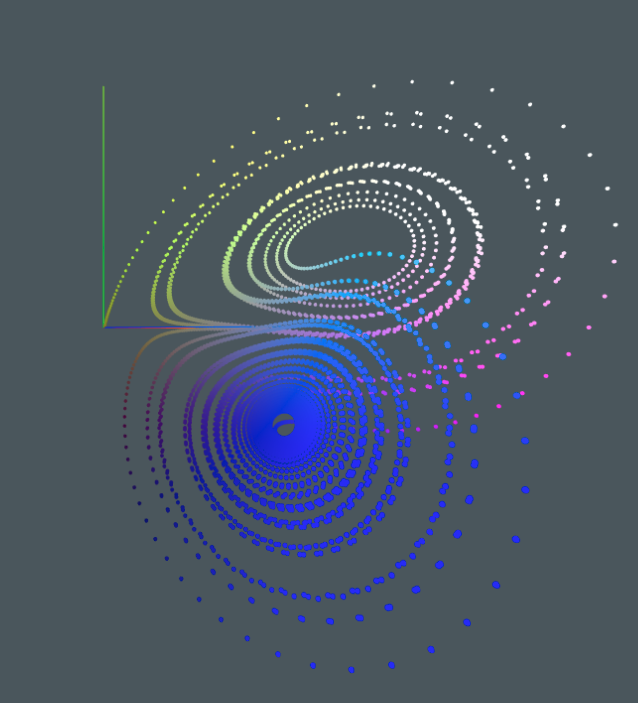
\includegraphics[width=0.7\linewidth]{../outline/lorenz-modell}
				\label{fig:lorenz-modell}
				\end{figure}
        	\end{column}
        \end{columns}
    \end{frame}
    
    \begin{frame}{Einführung Lorenz Attraktor}{Butterfly Effekt}
		\textit{"Predictability: Does the Flap of a Butterfly's Wings in Brazil Set Off a Tornado in Texas?"}, \\
		Paper Edward N. Lorenz, 1979
    \end{frame}
    
    \begin{frame}{Einführung Lorenz Attraktor}{Eigenschaften}
    	\begin{itemize}
    		\item Modell für Zirkulation der Atmosphäre auf der Erde
    		\item Zeigt, dass das Wetter chaotisches Verhalten hat
    		\item Näherung, keine verlässliche Vorhersage
    	\end{itemize}
    \end{frame}
    
    \begin{frame}{Einführung Lorenz Attraktor}{Was ist ein (strange) Attraktor?}
		
		\begin{columns}[c]
			\begin{column}{.6\textwidth}
				\begin{itemize}
					\item Menge von numerischen Werten, zu welchen ein System sich entwickelt
					\item Strange Attractor: Attraktor mit fraktaler Struktur
				\end{itemize}
			\end{column}
			\begin{column}{.4\textwidth}
				\begin{figure}
					\centering
					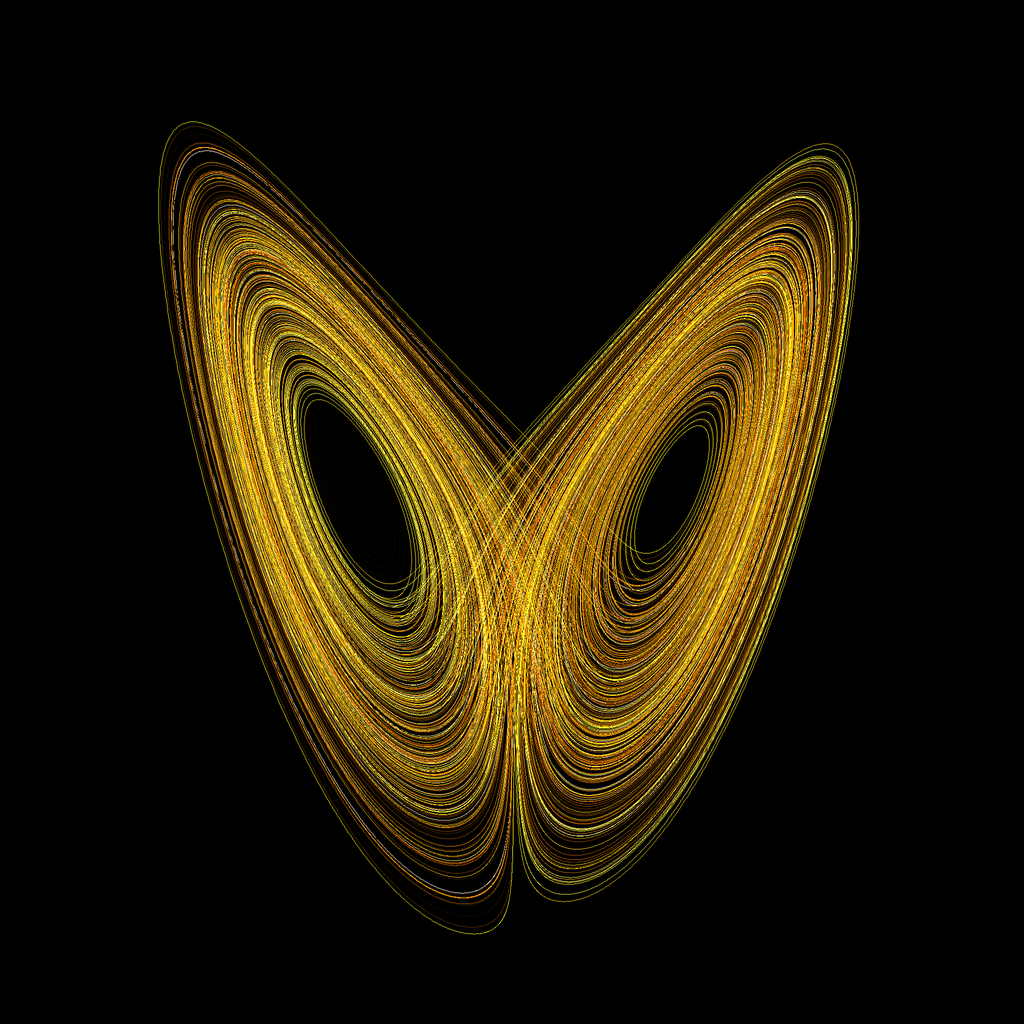
\includegraphics[width=1\linewidth]{Attractor}
					\label{fig:Attractor}
				\end{figure}
			\end{column}
		\end{columns}
    \end{frame}
    
	    
	\begin{frame}{Experiment zum Lorenz Attraktor}
		\begin{columns}[c]
			\begin{column}{.5\textwidth}
				\url{https://lorenz.olidias.ch}
			\end{column}
			\begin{column}{.5\textwidth}
				
\includegraphics[width=\textwidth]{olidiasQRCode}
			\end{column}
		\end{columns}
	\end{frame}
\end{document}